\chapter{コンテンツ視聴時に生体データを取得しコンテンツへ重畳提示}

\thispagestyle{myheadings}

\section{提案手法}

\subsection{システム構成}
図1に研究の全体像を示す.システムの流れはコンテンツを視聴しているときの生体データを取得し,サーバにアップロードする。生体データはコンテンツ毎に収集する.集めた生体データから盛り上がっている箇所を推定し,抜き出す.抜き出したデータを基にコンテンツに重畳表示するといった構成である.
\begin{figure}[H]
    \centering
    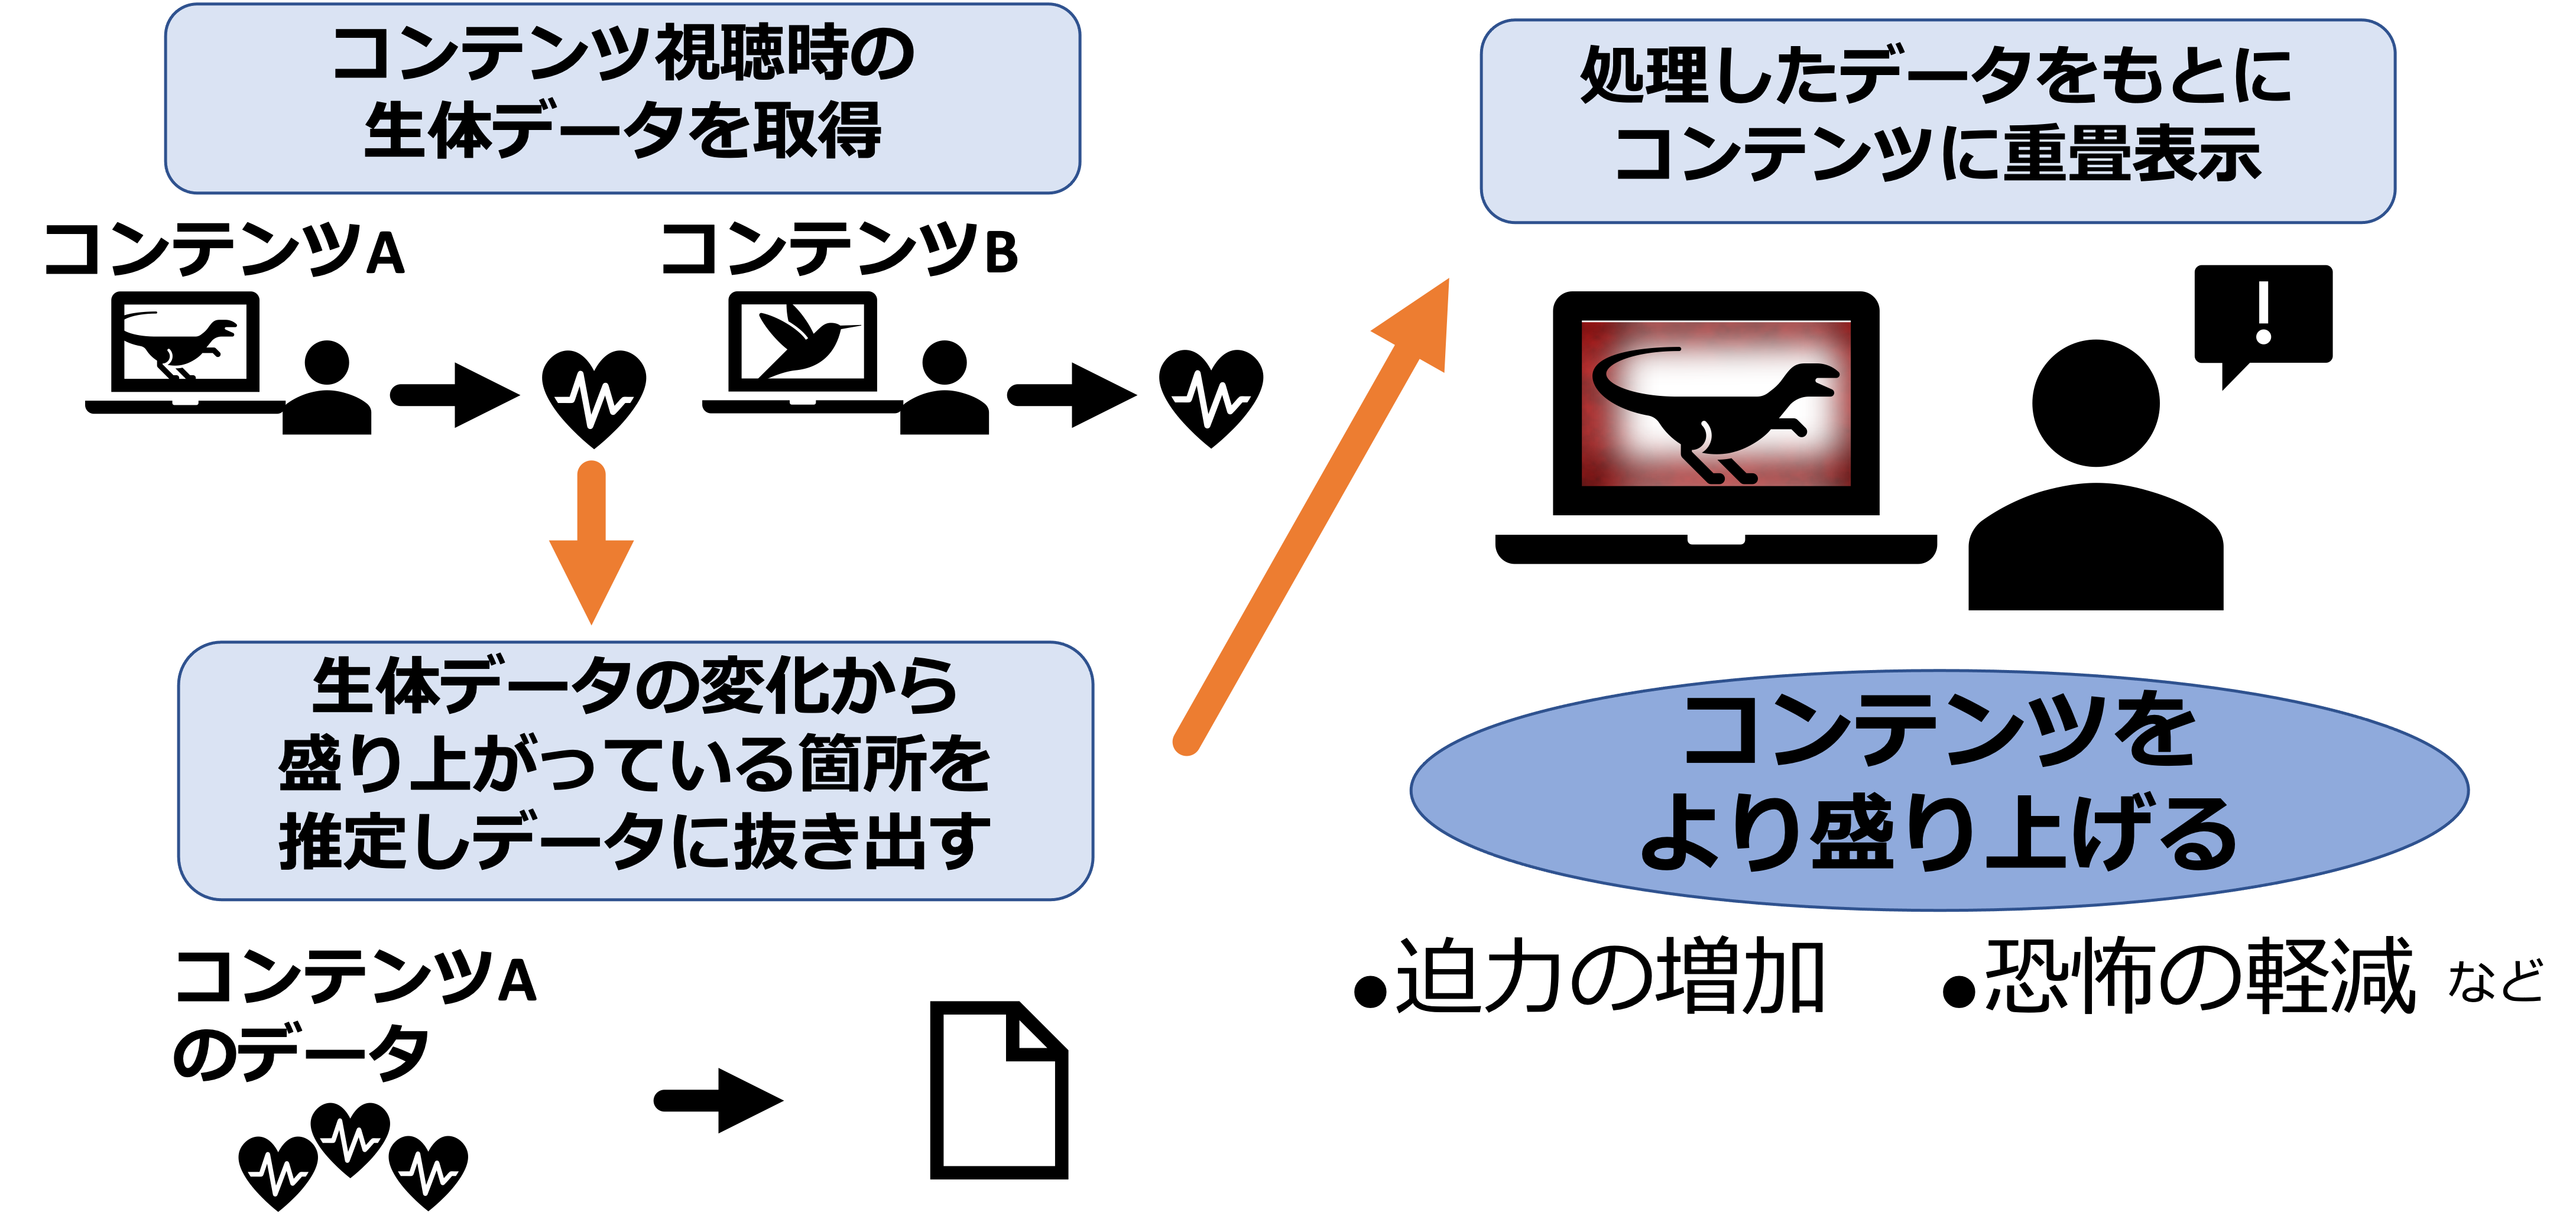
\includegraphics[width=10cm]{images/chapter3/zenntaizu.png}
    \caption{システム全体図}
\end{figure}
生体データとして目の動きに注目したり,額から出る汗の量でコンテンツ視聴時の興奮度を測る方法などが考えられる.収集する生体データによってコンテンツに対し盛り上がり方を色々な目線で計測が可能である.コンテンツへの重畳方法も音を追加して迫力を増したり,画面にエフェクトを表示や振動させたりなどさまざまである,生体データ,重畳方法ともに多岐に渡り用途を決めるのが可能である.

\subsection{本研究のシステム構成}
本研究で採用したシステムについて述べる.本研究では生体データの収集方法としてスマートウォッチを採用した.理由として近年スマートウォッチは普及しており,誰でも気軽に生体データを取得できるからである.今回スマートウォッチはTicWatchE3を利用した図.生体データとして心拍数を計測する.スマートウォッチを使い気軽に計測ができるためである.スマートウォッチで心拍数を計測するためAndroidStudioで心拍数が収集できるアプリを作成した.コンテンツは映画を視聴するようにした.コロナ禍により自宅で映画を見る機会が増えたためである.また,映画は盛り上がるポイントが明確に出てくると予想したからである.映画にはエフェクトを重畳する.映画画面に直接エフェクトを表示しで迫力や恐怖などを体験できると考えたからである.本研究の流れは映画を見ている時の心拍数をスマートウォッチを使って計測し,取得したデータを心拍数が上昇している箇所のみのデータにする.そのデータを基に映画画面にエフェクトを重畳するという流れになっている.
\begin{figure}[H]
    \centering
    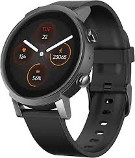
\includegraphics[width=10cm]{images/chapter3/tokei.jpg}
    \caption{利用したスマートウォッチ,TicWatchE3}
\end{figure}

\begin{figure}[H]
    \centering
    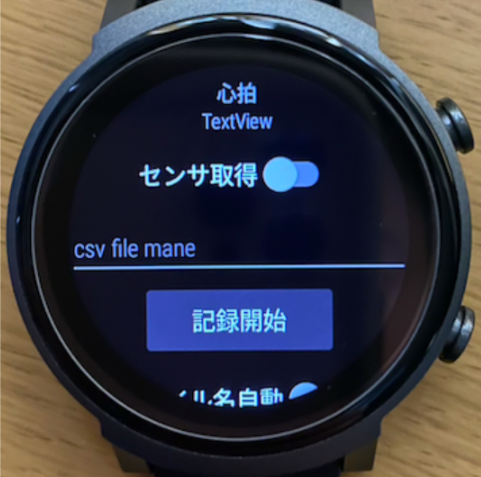
\includegraphics[width=10cm]{images/chapter3/tokei_real.png}
    \caption{心拍数取得画面}
\end{figure}

\section{心拍データの分析と心拍上昇箇所の抽出処理}
収集した心拍数のデータを分析した.実際に集めたデータをグラフにしたものを表示する.映画は「キングコング」を視聴した人のデータである.集めたデータを観察したところ,人により心拍数の変動が様々であった.図のように常に心拍数が上昇と下降を繰り返している人や,盛り上がりを見せるシーンでは心拍数が大幅に上昇し,それ以外は上昇と下降を繰り返している人,また盛り上がりを見せるシーンのみ心拍数が上昇しそれ以外は比較的落ち着いている人などがいた.
\begin{figure}[H]
    \centering
    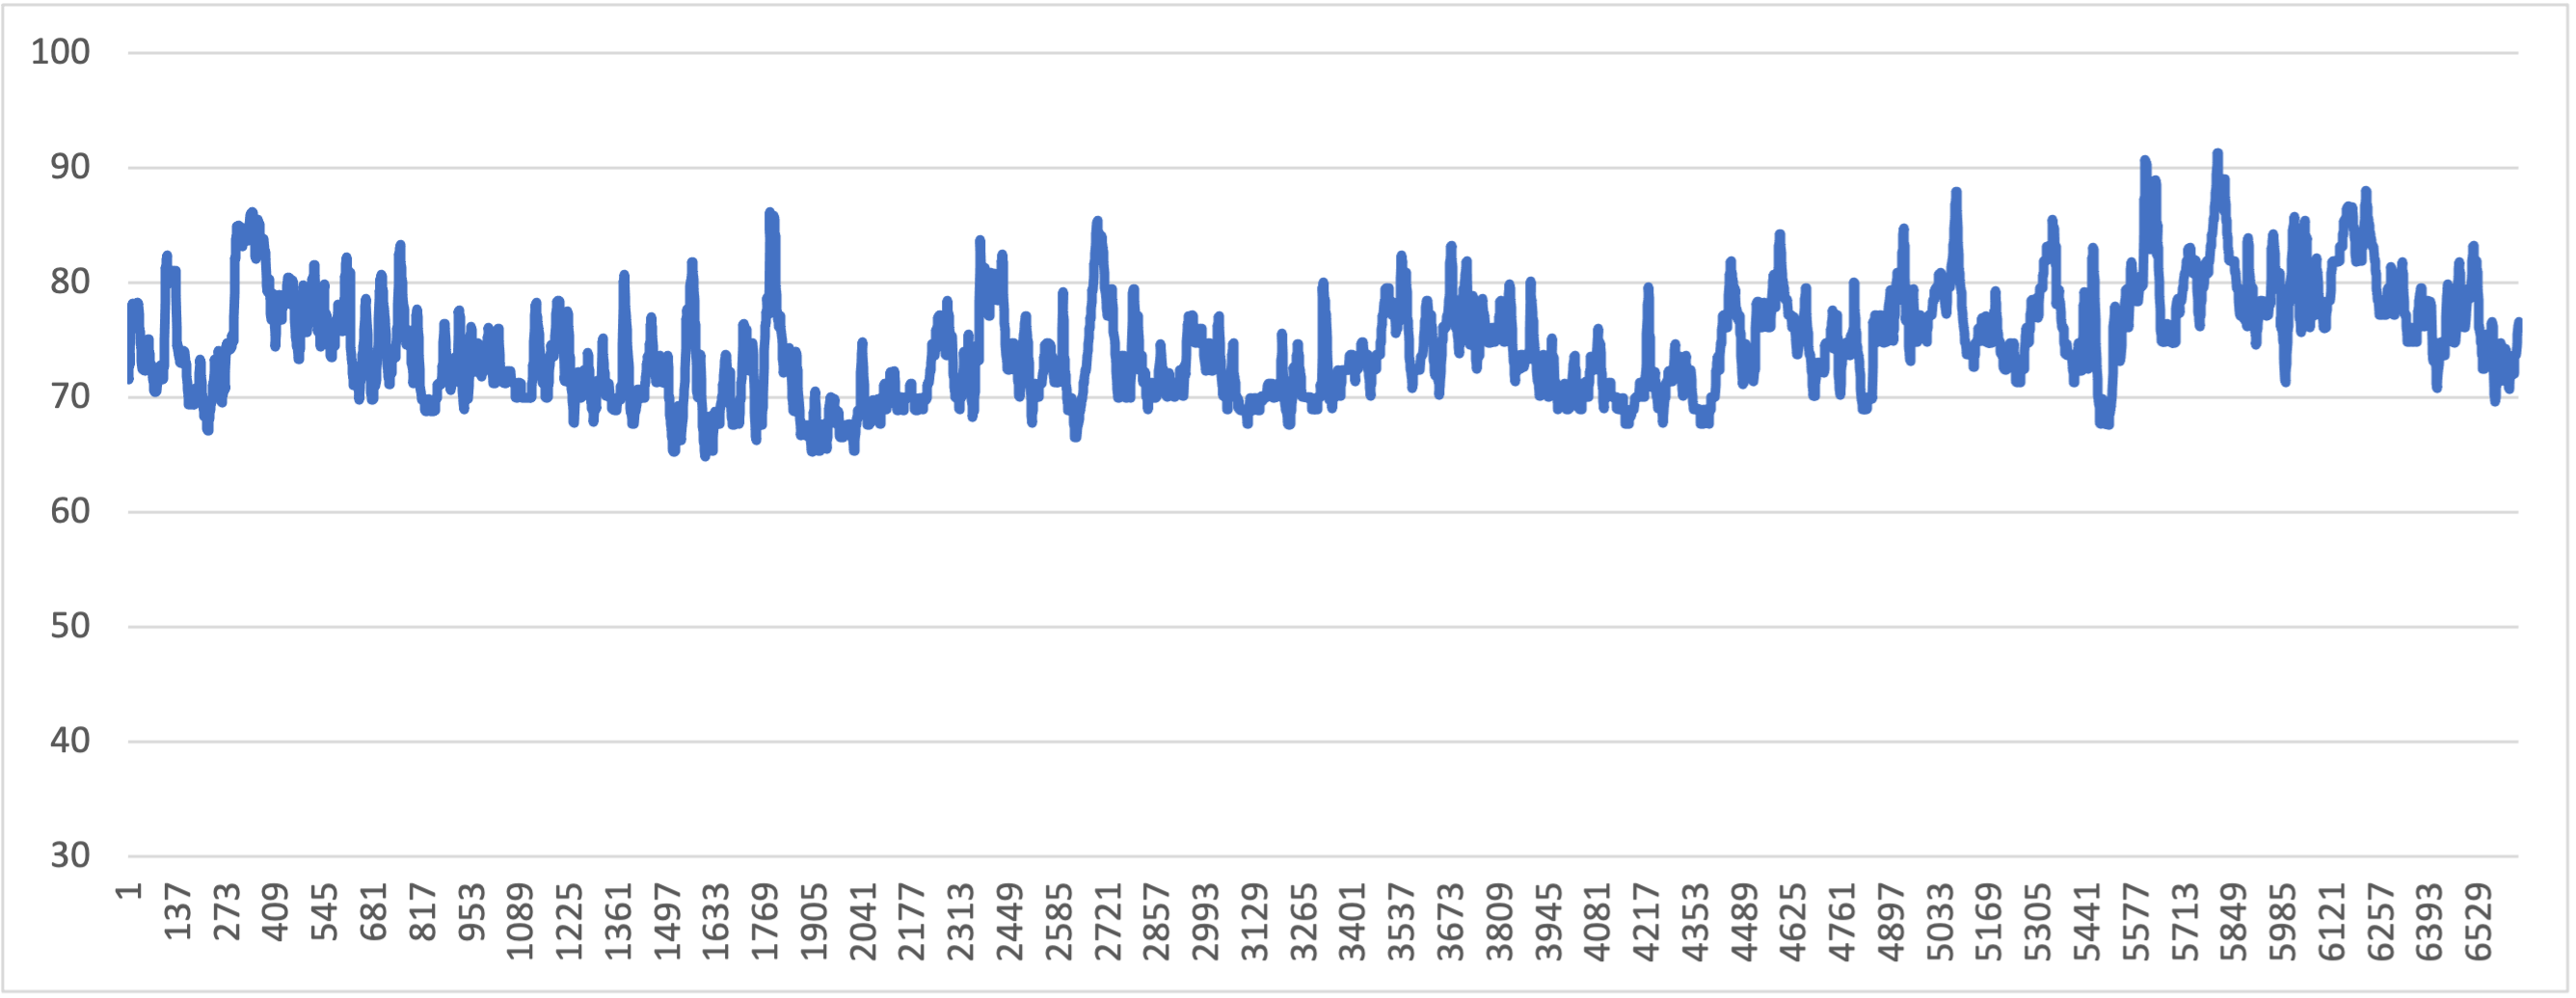
\includegraphics[width=10cm]{images/chapter3/gurafu1.png}
\end{figure}

\begin{figure}[H]
    \centering
    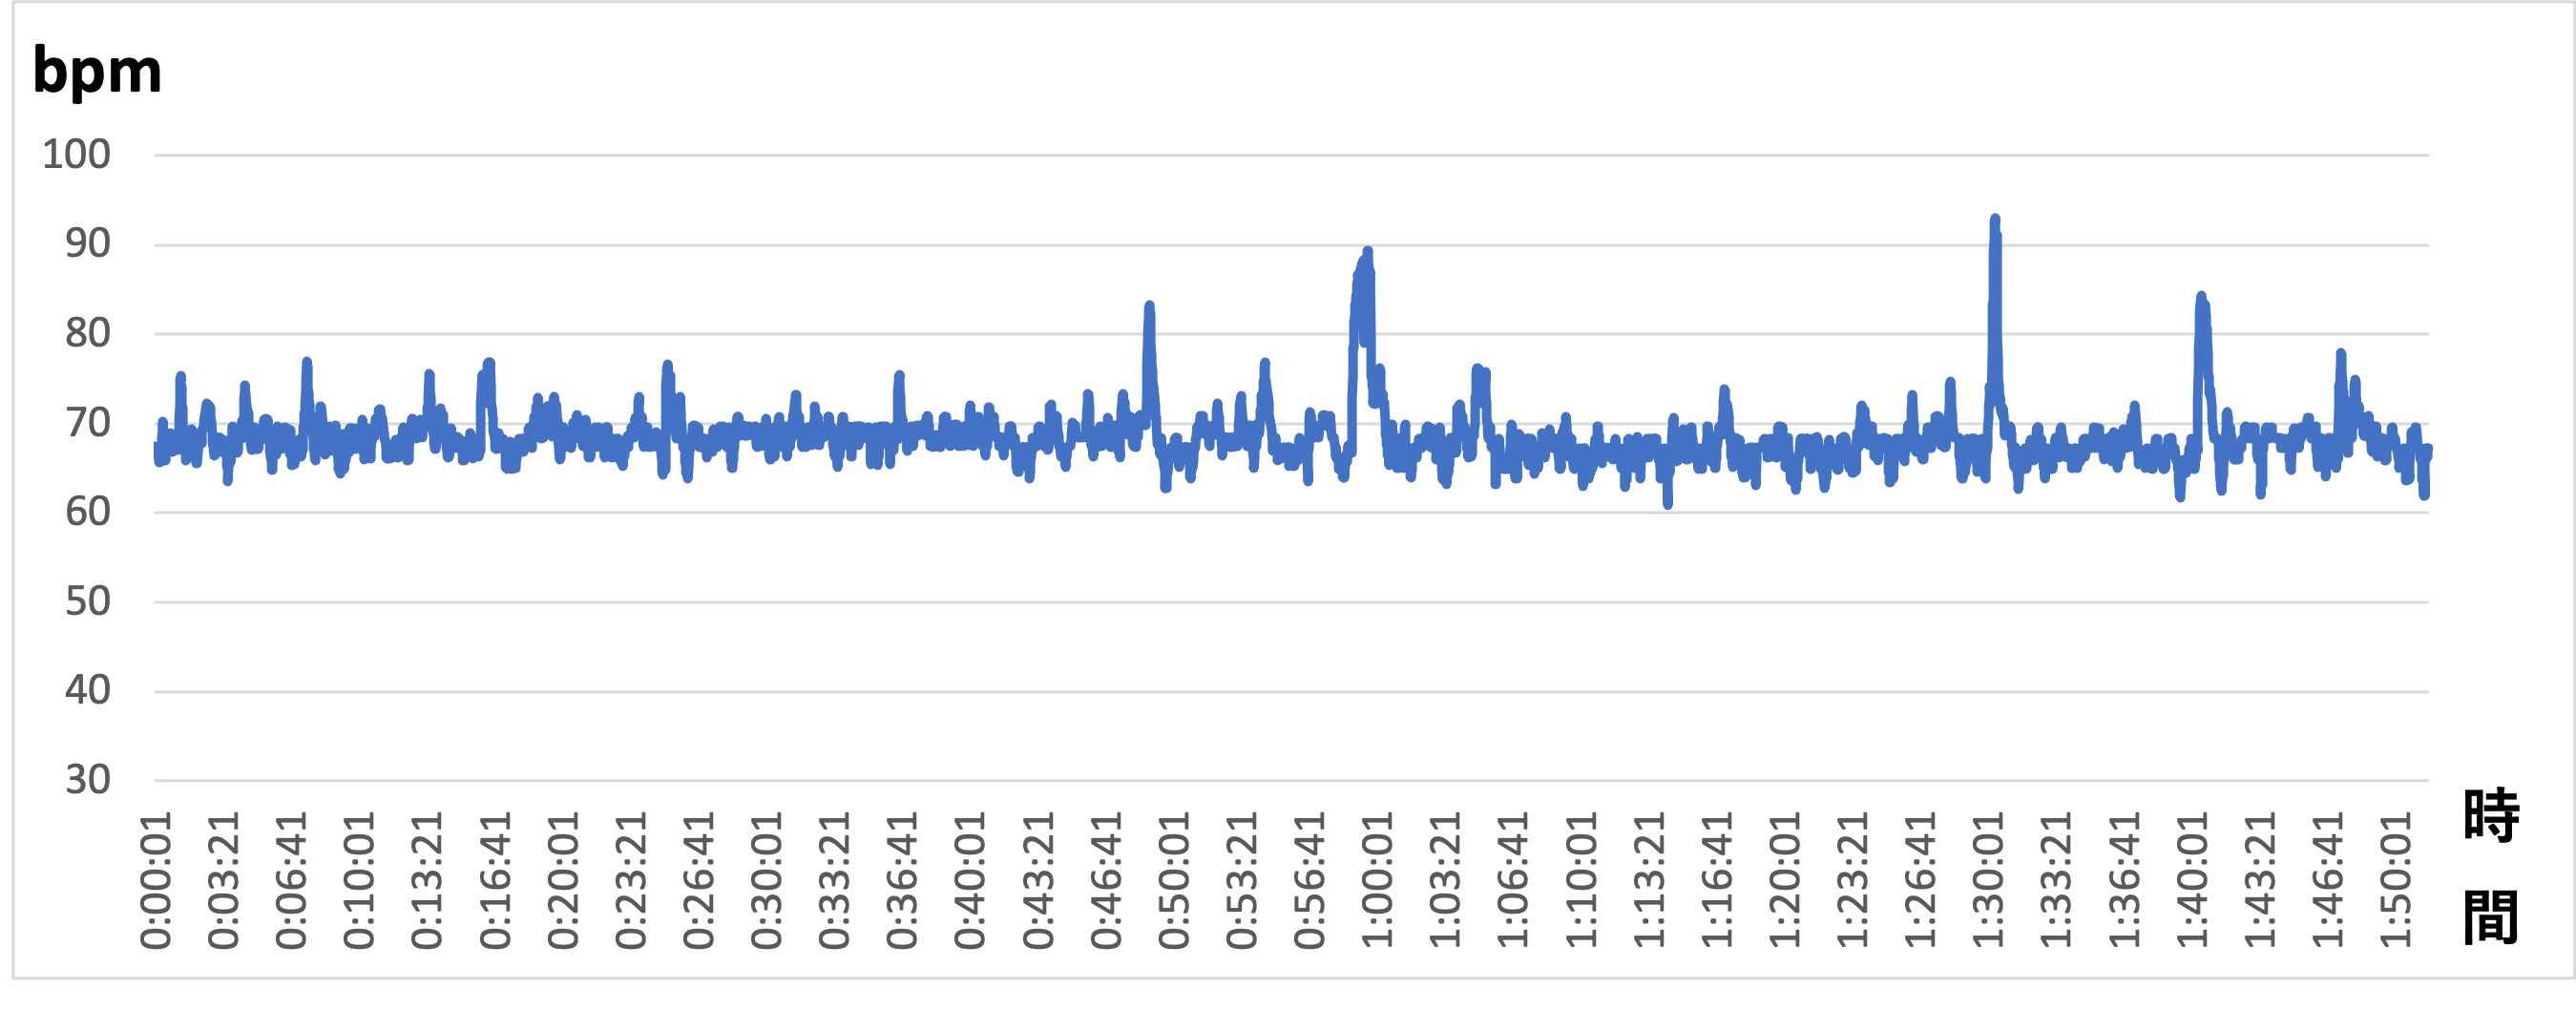
\includegraphics[width=10cm]{images/chapter3/gurafu2.png}
\end{figure}

\begin{figure}[H]
    \centering
    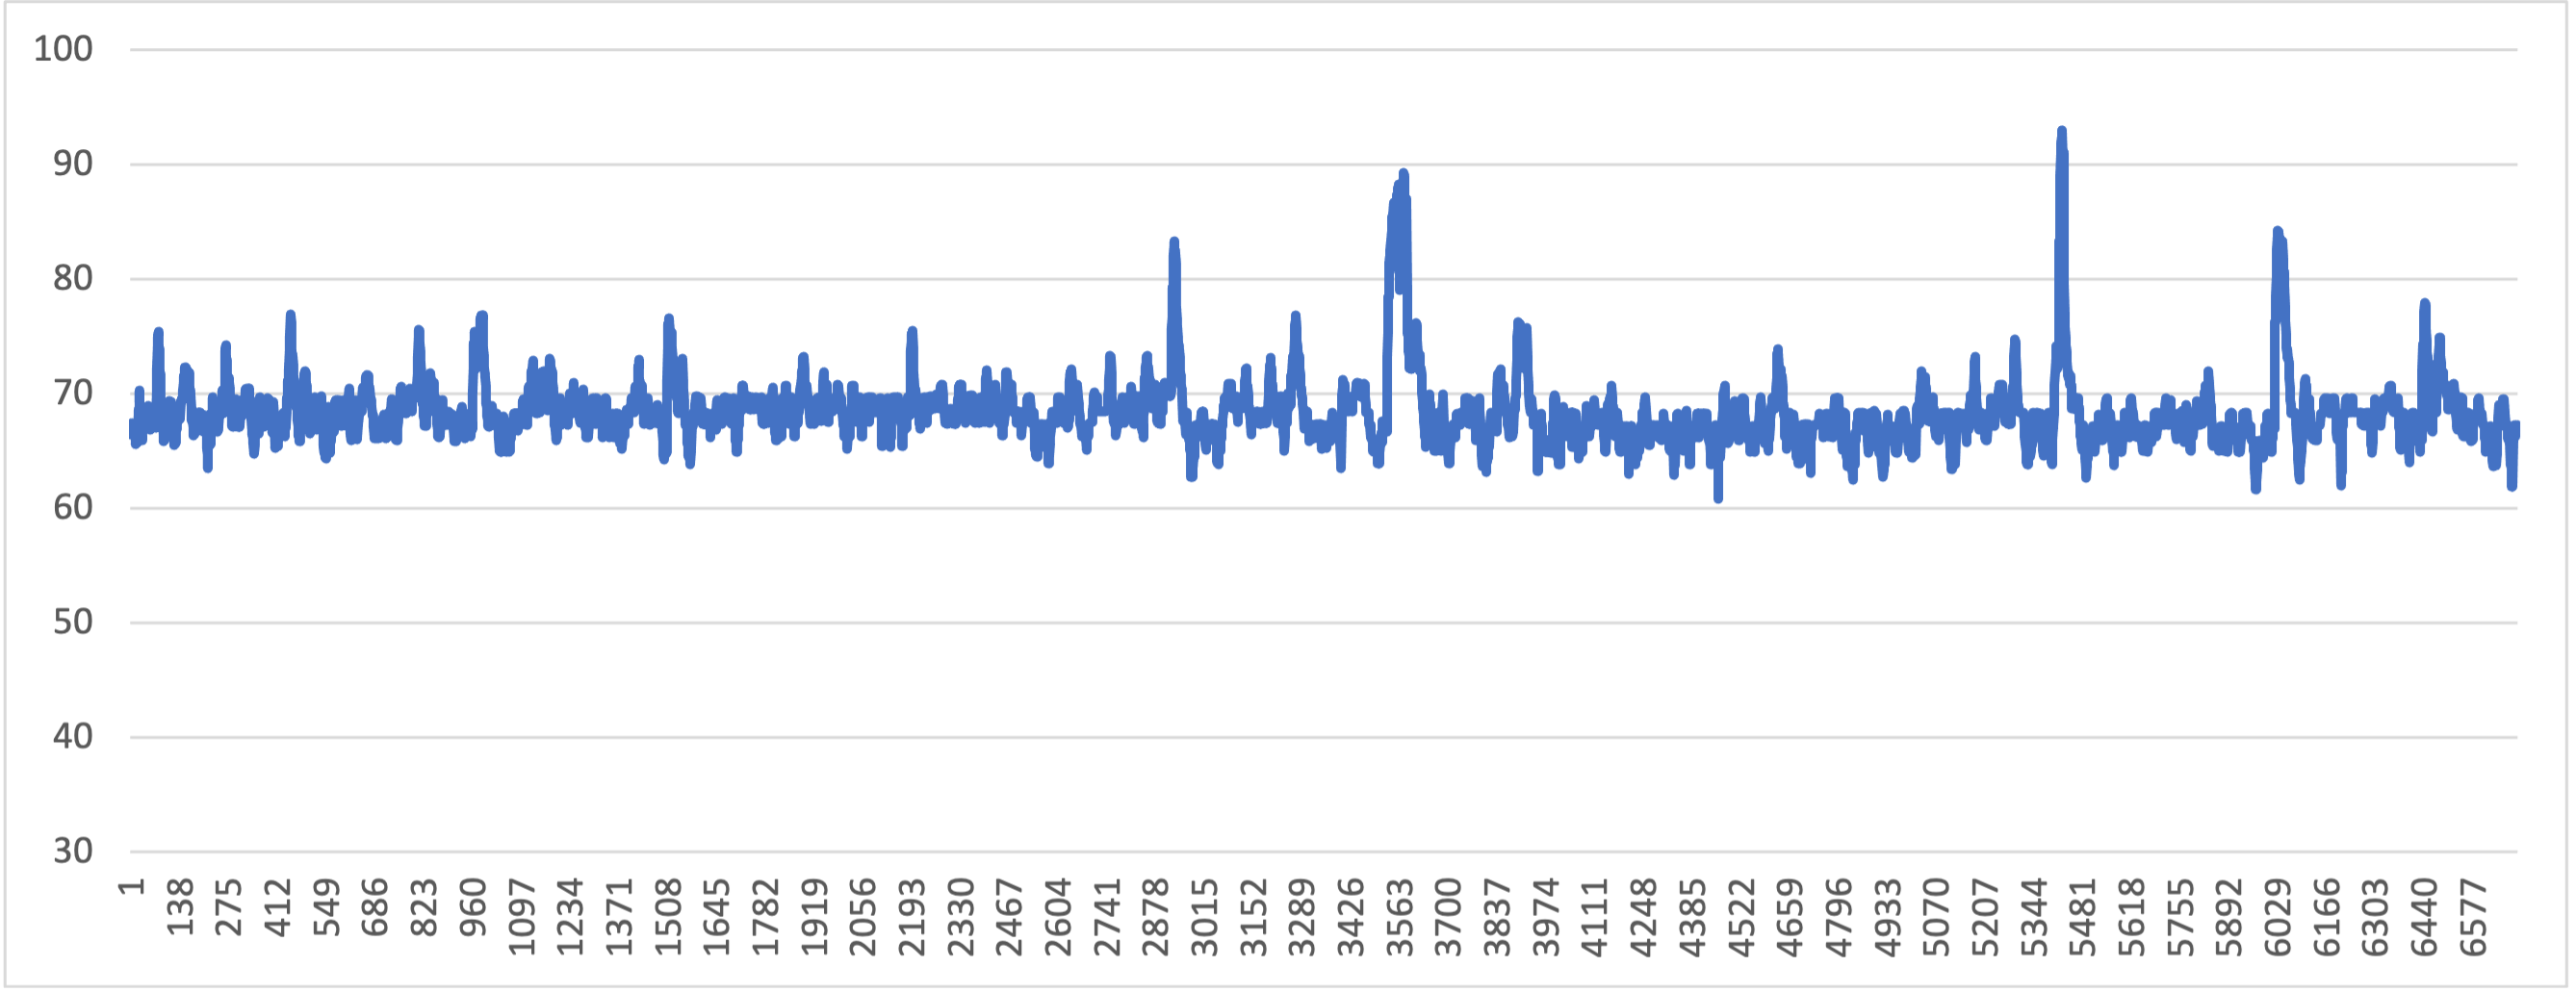
\includegraphics[width=10cm]{images/chapter3/gurafu3.png}
    \caption{キングコングを視聴した時の心拍数のグラフ}
\end{figure}

エフェクト表示に適した形式にするため,心拍上昇箇所の抽出処理方法を述べる.映画の盛り上がりのシーンを抜き出すため,心拍数が上昇している箇所を抽出する.収集した心拍数の CSV データを心拍上昇箇所のみのJSON データにする.抽出処理の方法を図 に示す.スマートウォッチで収集した心拍数のデータはcsvファイルとしてサーバにアップロードされる.サーバからデータ毎に心拍数上昇箇所の抽出を行い,上昇した箇所のみのjsonデータにする.心拍数が上昇しているところを抜き出すため,安静時の心拍数からどれだけ心拍数が上昇したかを抽出する.まず映画を見る前の1分間を安静時の心拍数として平均を出し閾値にする. 次に図のように心拍 数を閾値と比較する.心拍数の上昇具合で表示するエフェクトを変更するため,1 から 3 までのレベル分けをした.平均心拍数よりも心拍数が 16bpm 以上高い時を レベル 3,14bmp 以上をレベル2,12bpm 以上をレベル 1 とする.from to の形式で心拍数が閾値を超えていた 時間を示す.時間は映画が始まってからの経過時間で エフェクトを表示するため相対時間にした.effectlevel で表示するエフェクトを決定する。実際に心拍数上昇箇所の抽出処理をした後のデータを図に示す.エフェクトの表示に適した形式にするため,心拍上昇箇所の抽出処理した JSON データを一つの JSON データにまとめる.これにより一つのコンテンツに一個の JSON データが作られる.このデータを使いエフェクトを映画画面に重畳する.

\begin{figure}[H]
    \centering
    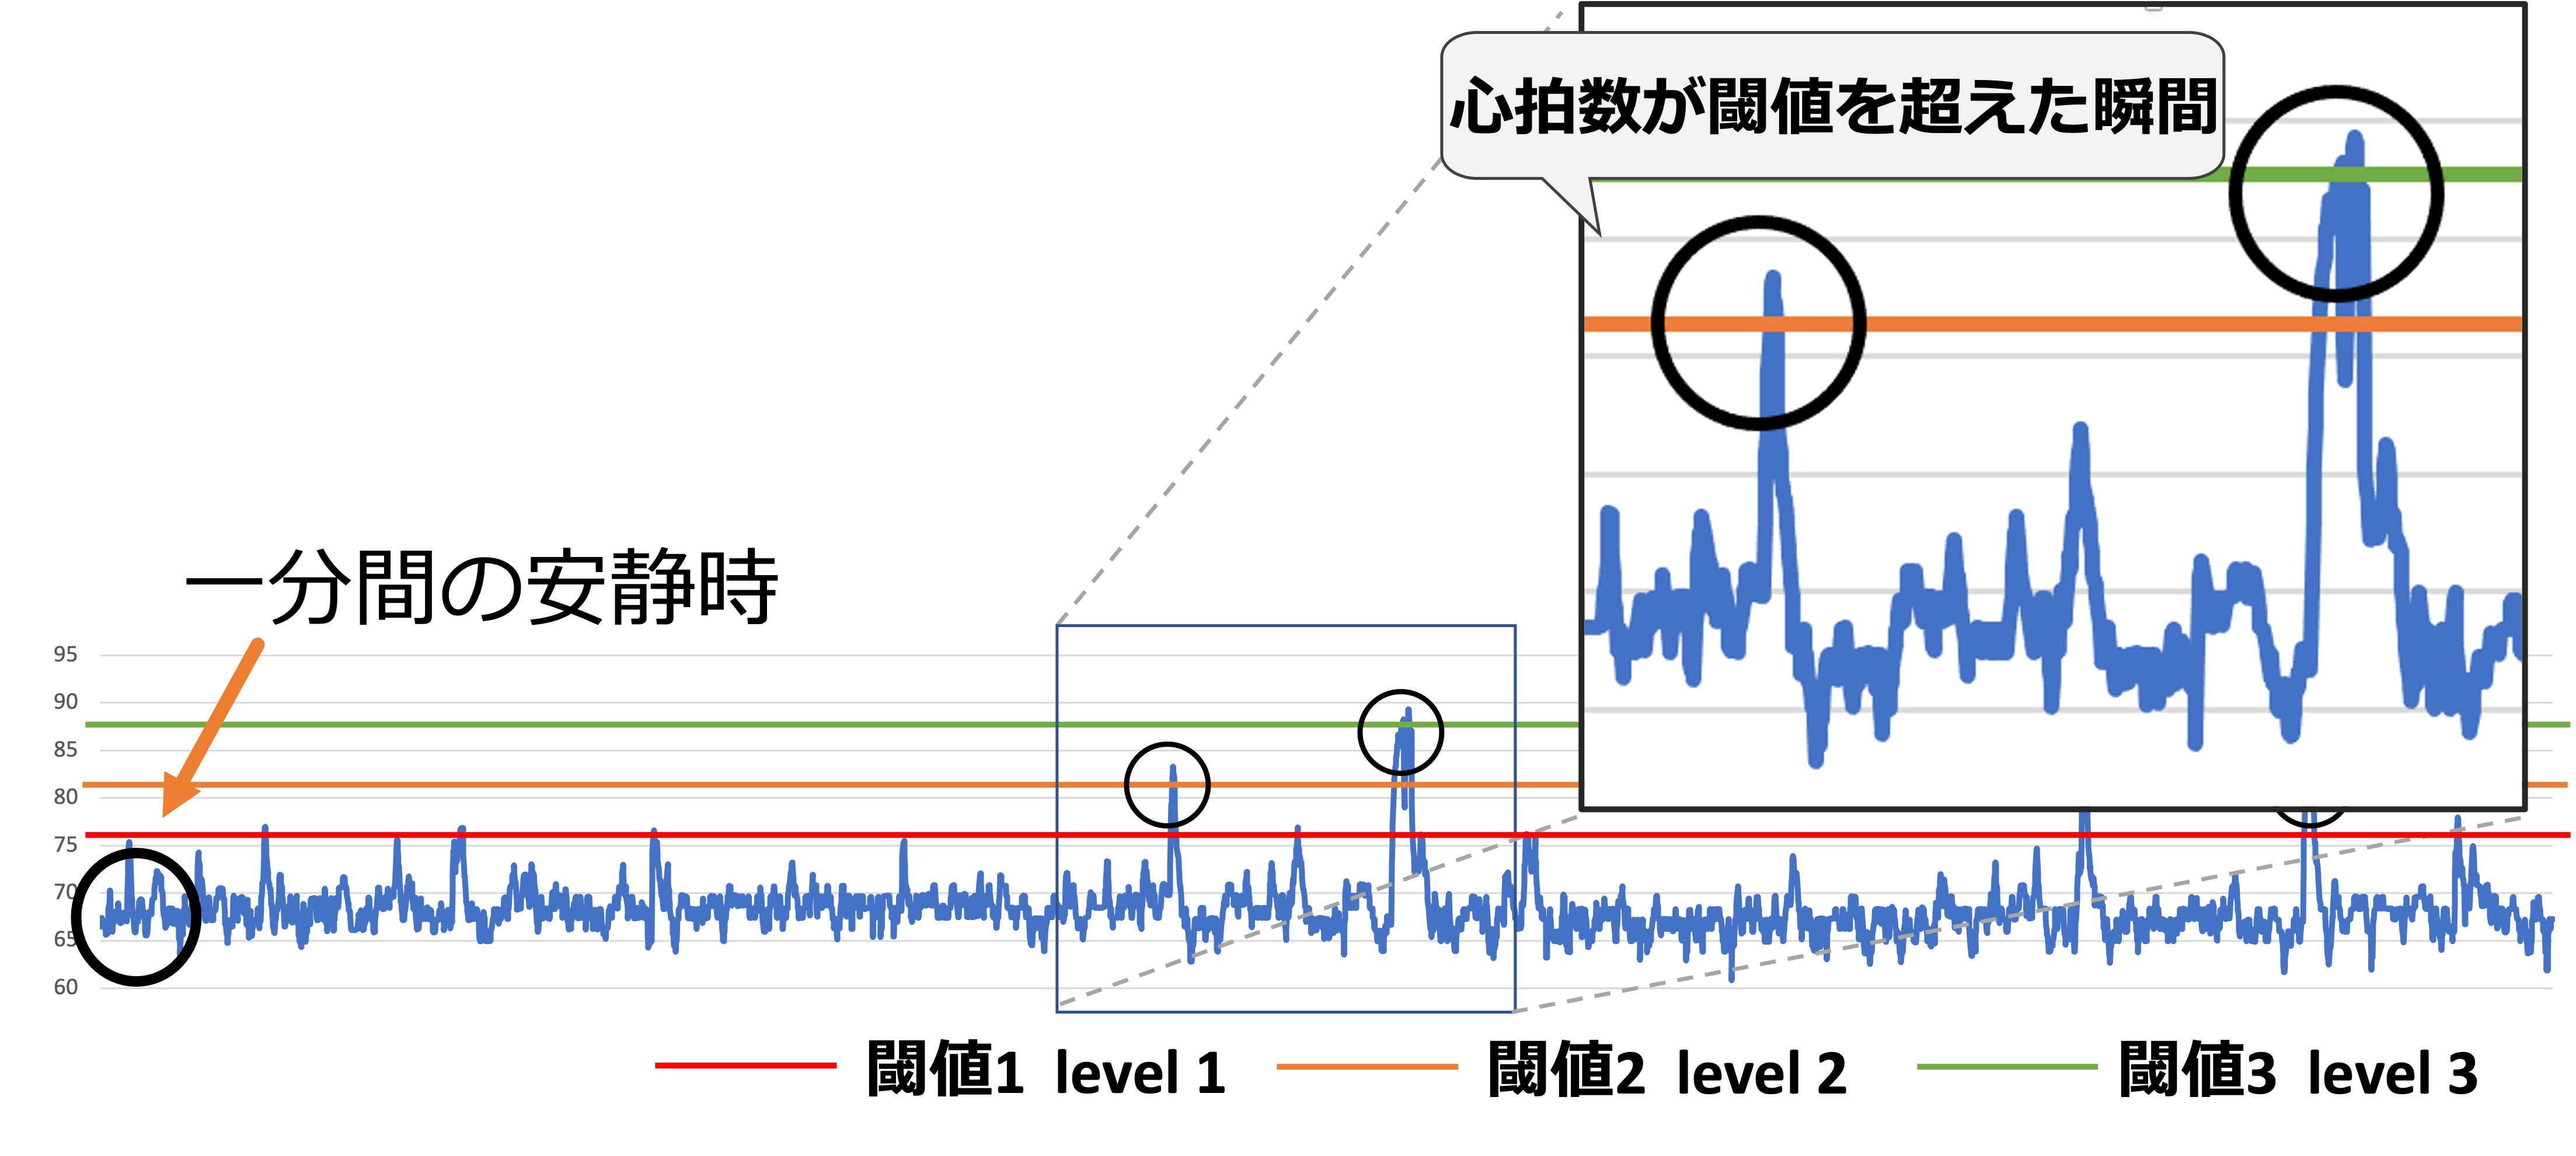
\includegraphics[width=10cm]{images/chapter3/haisyutusyori.png}
    \caption{心拍数上昇箇所の抽出処理}
\end{figure}

\begin{figure}[H]
    \centering
    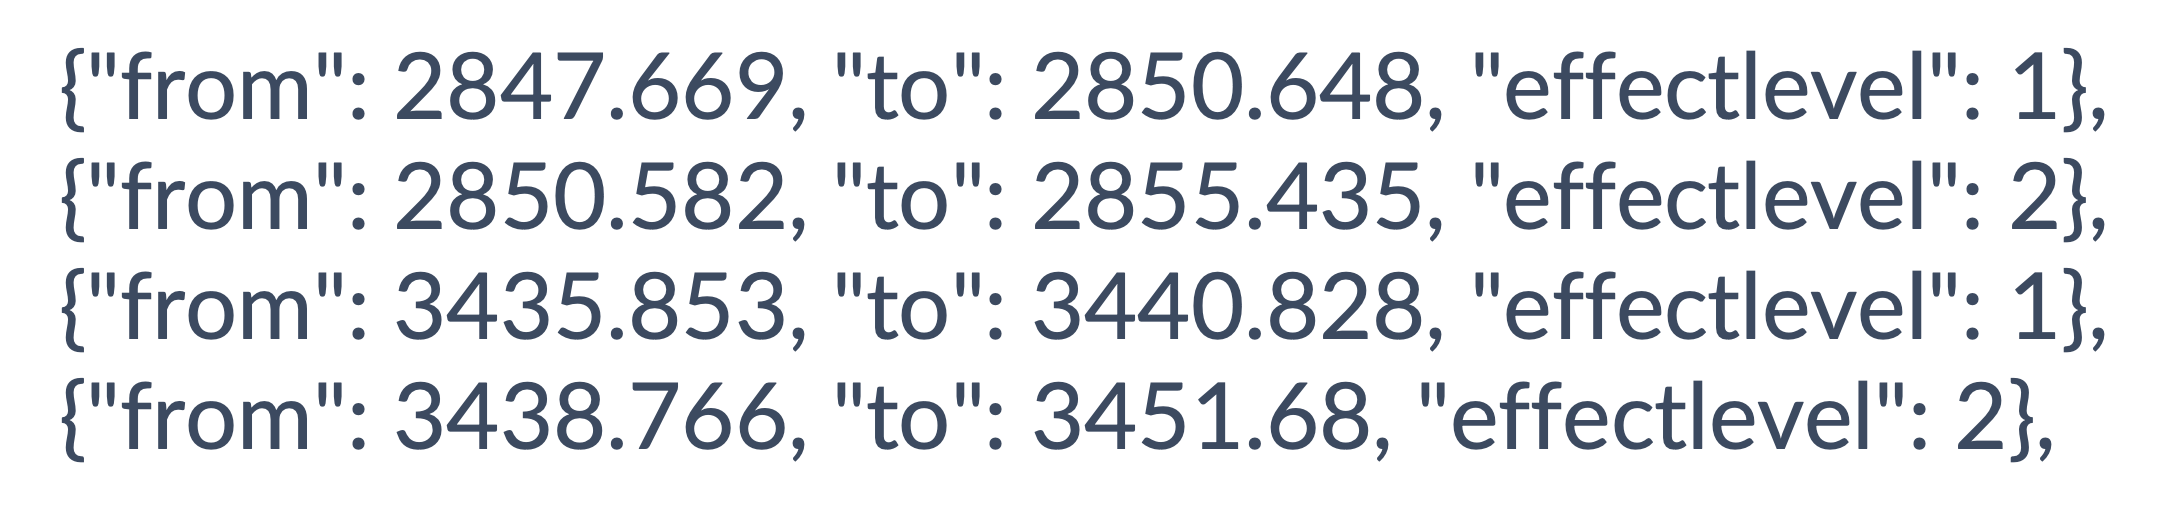
\includegraphics[width=10cm]{images/chapter3/level.png}
    \caption{心拍数上昇箇所の抽出処理をした結果}
\end{figure}

\section{エフェクト表示}
\subsection{本研究のシステム構成}
エフェクト表示方法として,カテゴリやレベルごとにエフェクトを用意し,動画として重畳表示しているが,レベル分けを行ったためエフェクトをダイナミックに生成できず,細かな心拍数変化を表示できていない.
本研究では,視聴者ごとにエフェクトを自由に選択できるようにするためElectronを使用し,PCを使用する環境下での重畳表示が可能になっている.
Electronを起動し,視聴する動画コンテンツを選択し,視聴する映画のジャンルに合わせるエフェクトを選択し,Playをクリックし,エフェクト重畳が開始するようになっている.実際の動作画面を図に示す.

\begin{figure}[H]
    \centering
    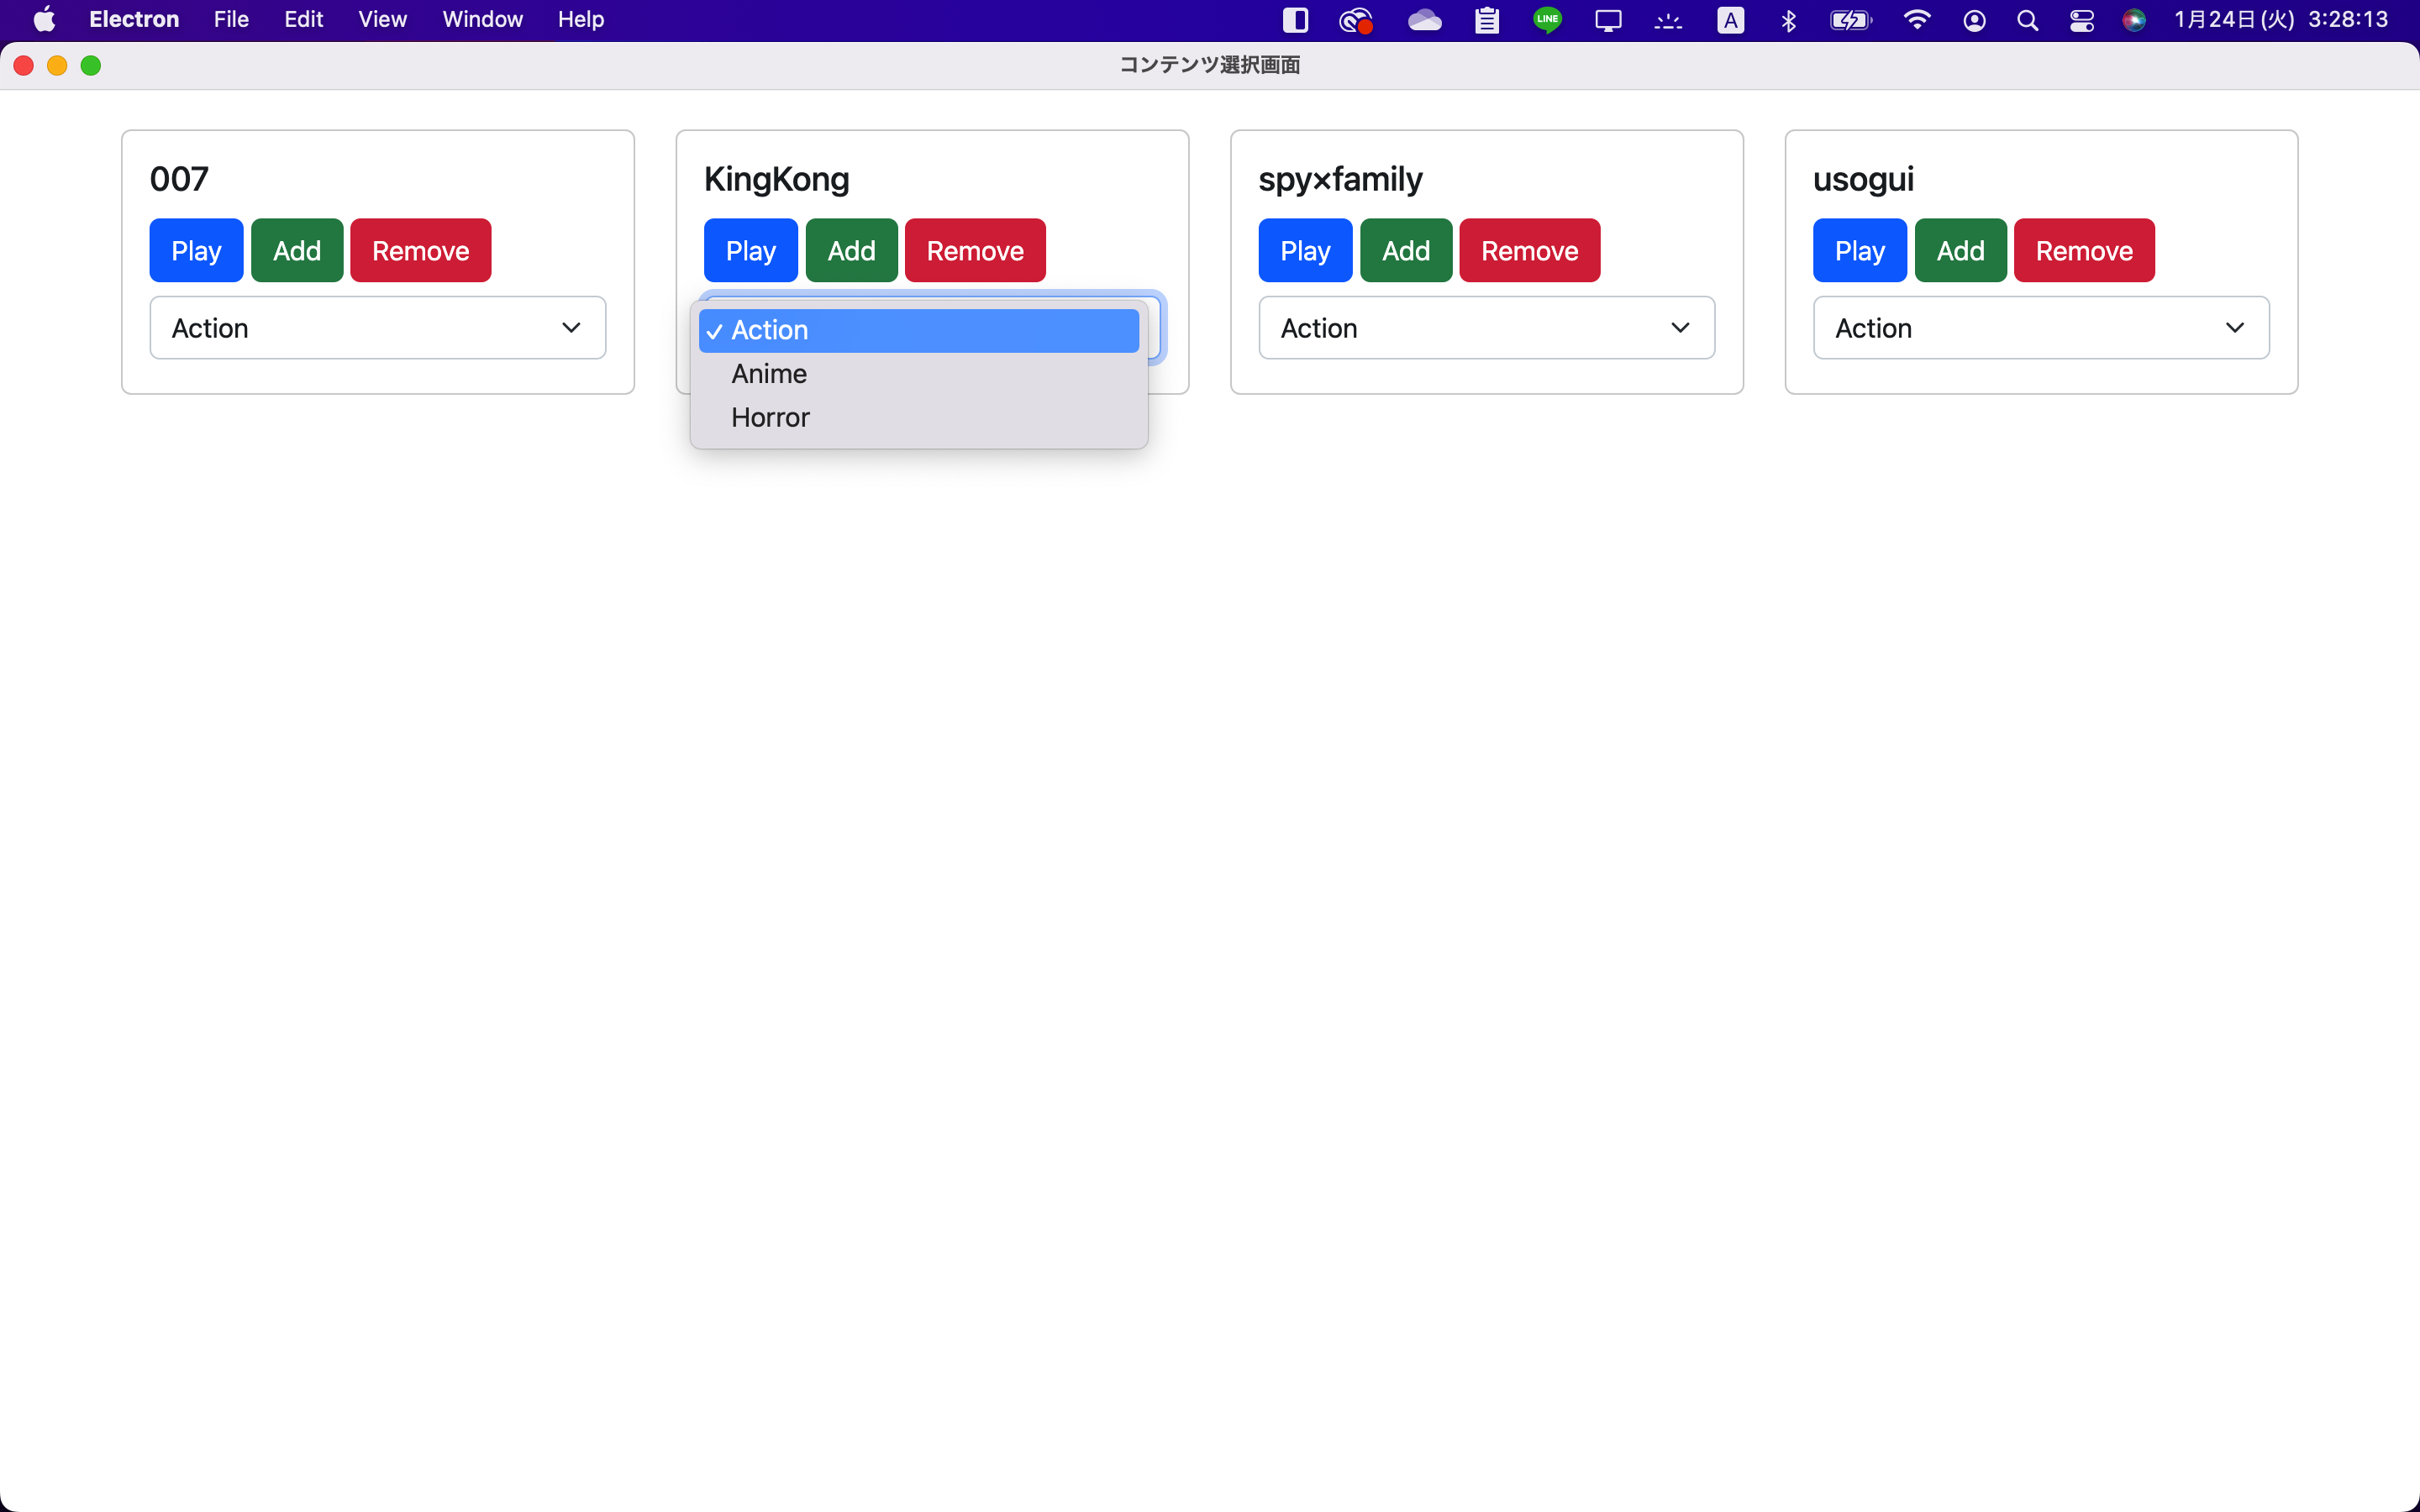
\includegraphics[width=10cm]{images/chapter3/contents.jpg}
    \caption{コンテンツ選択画面}
\end{figure}

\subsection{エフェクト種類}
エフェクトの種類としてAction, Anime, Horrorの3種類に分け見る映画のジャンルを選択可能にした.選択できるようにした理由として,視聴ジャンルによって同じエフェクト効果を表示した際に,エフェクトが映像視聴の際に邪魔になってしまう点が挙げられる.
エフェクトの目的として,Actionのエフェクトは迫力・緊迫感を与え,Animeのエフェクトは面白さを与える,Horrorのエフェクトは恐怖を軽減させる目的として制作した.心拍データの処理の際に1から3までのレベル分けの結果でエフェクトが変更される.1から3に分けた際に1の結果が出力された時間はエフェクトを透過し映像視聴の邪魔にならないように制作し,2と3の結果が出力されている時のみに2段階に分けエフェクトが表示されるように制作した.
実際の画面にエフェクトを表示した例を図に示す,Actionのエフェクトは赤色の不透明度を上げ,色相彩度を上げる.Animeのエフェクトは効果線を増やす.Horrorのエフェクトは不透明度を下げ,ぼかしの不透明度を上げるように制作した.Action, Horrorのエフェクト制作ではAfter Effectsを使用しフラクタルノイズ効果,色被り補正で制作.Animeのエフェクト制作ではIllustratorを使用し効果線を制作した.

\begin{figure}[H]
    \centering
    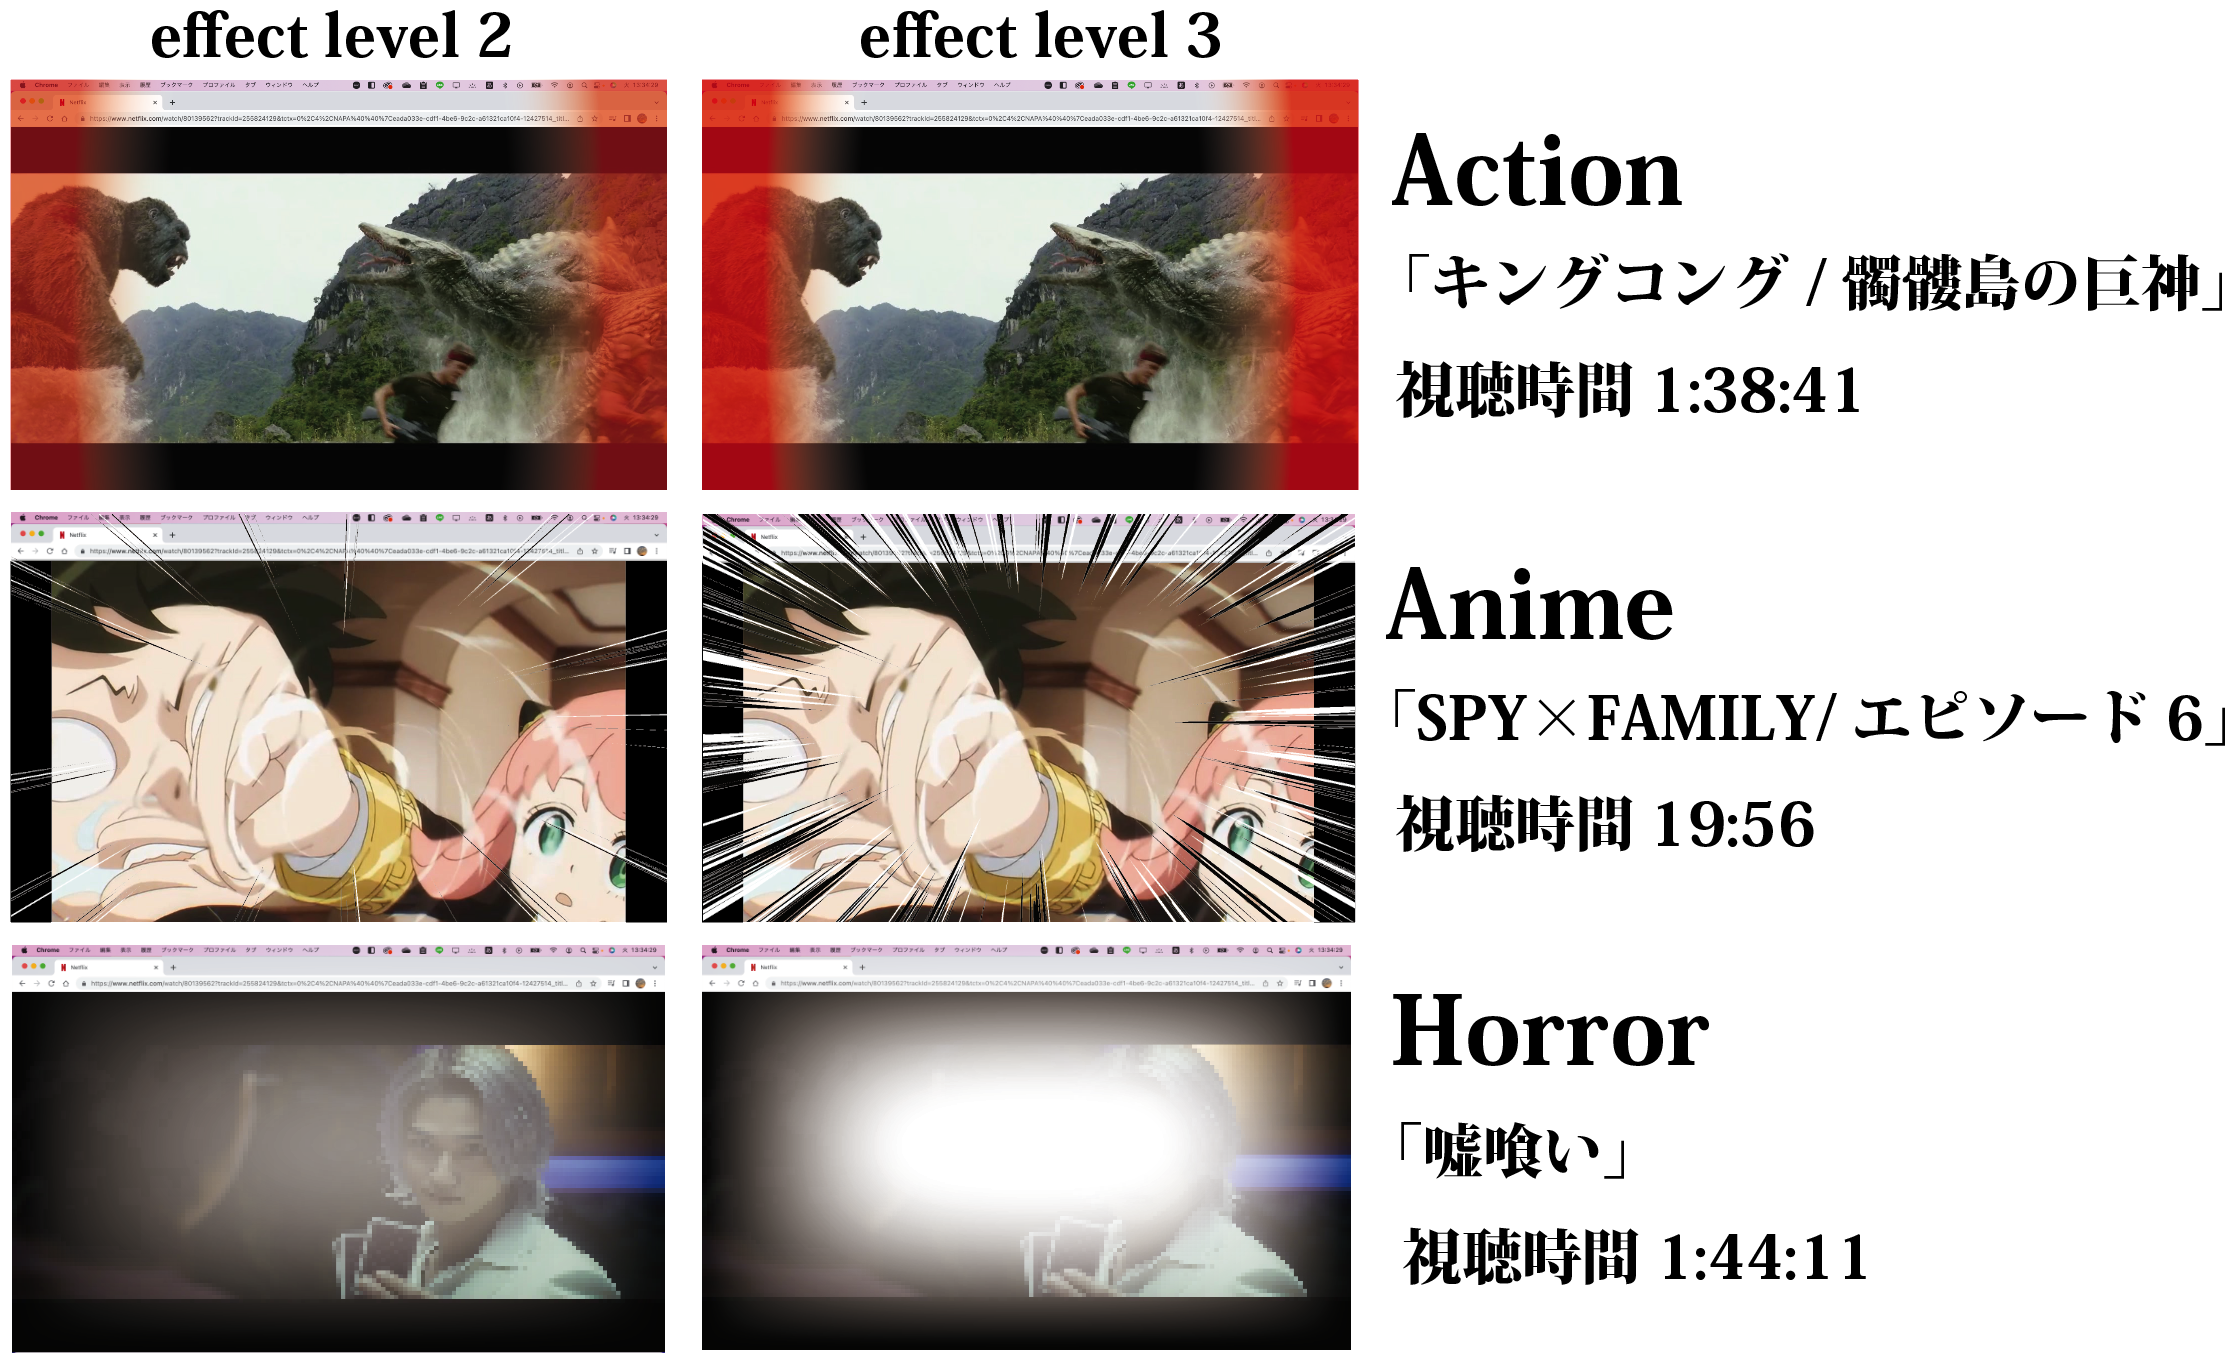
\includegraphics[width=10cm]{images/chapter3/effectjissou.jpg}
    \caption{実装画面}
\end{figure}